\documentclass[t]{beamer}
\usetheme{default}
\usecolortheme{default}
\usepackage{macros}


\begin{document}
\begin{frame}
    \frametitle{Overview}
    \begin{block}{Goal}
        Constrain the high mass ($\FullMstar{} \gtrsim{} 11.5$) satellite fraction (\fsat{}) in Hyper Suprime-Cam (HSC) observations.
    \end{block}

    \begin{block}{How}
        \begin{itemize}
            \item In an N-body simulation, map some halo property (\eg{} \MhaloPeak{}, \vmp{}) to \Mstar{}, with some scatter.
            \item Optimize this mapping in to fit some HSC observations (\eg{} SMF, clustering).
            \item Measure \fsat{} in the best fitting mock.
        \end{itemize}
    \end{block}

    \begin{block}{See also}
        Reddick 2013 did this for SDSS
    \end{block}
\end{frame}

\begin{frame}
    \frametitle{Observations + Simulation data}

    \begin{columns}

    \column{0.5\textwidth}
    \begin{block}{Hyper Suprime Cam}
        \begin{itemize}
            \item $\sim{}$4500, 30 $\FullMstar > 11.5,\ 12$
            \item $z \sim{} 0.3$ (check)
        \end{itemize}
    \end{block}

    \column{0.5\textwidth}
    \begin{block}{MDPL}
        \begin{itemize}
            \item 1000 $\Mpc{}\, \h{}$
            \item Snapshot at $z \sim{} 0.37$
        \end{itemize}
    \end{block}

    \end{columns}

\end{frame}

\begin{frame}
    \frametitle{Fitting choices}

    \begin{block}{Halo Parameter}
        $\Mstar{} = f({\rm halo\, property})$. We build models with \vmp{} and \MhaloPeak{}.
    \end{block}

    \begin{block}{Functional form}
        We use Behroozi + halo mass dependent scatter (linear). Other options were an HOD, abundance matching.
    \end{block}

    \begin{block}{Fitting Data}
        \begin{itemize}
            \item The SMF
            \item Counts in cylinders: $\xi(r_p, r_{\pi})$ in a single $r$ ($< 1\Mpc$) and $\pi$ ($< 10\Mpc$) bin. HSC doesn't have enough data for a more detailed measurement of clustering. This is a cross correlation between galaxies $\FullMstar > M$ and $M - 0.1 < \FullMstar < M$ for a couple of $M$.
        \end{itemize}
    \end{block}

\end{frame}


\begin{frame}
    \frametitle{Bestfit Models 1: SMF}

    \begin{columns}
    \column{0.5\textwidth}

    \begin{block}{\vmp{}}
        \begin{figure}
        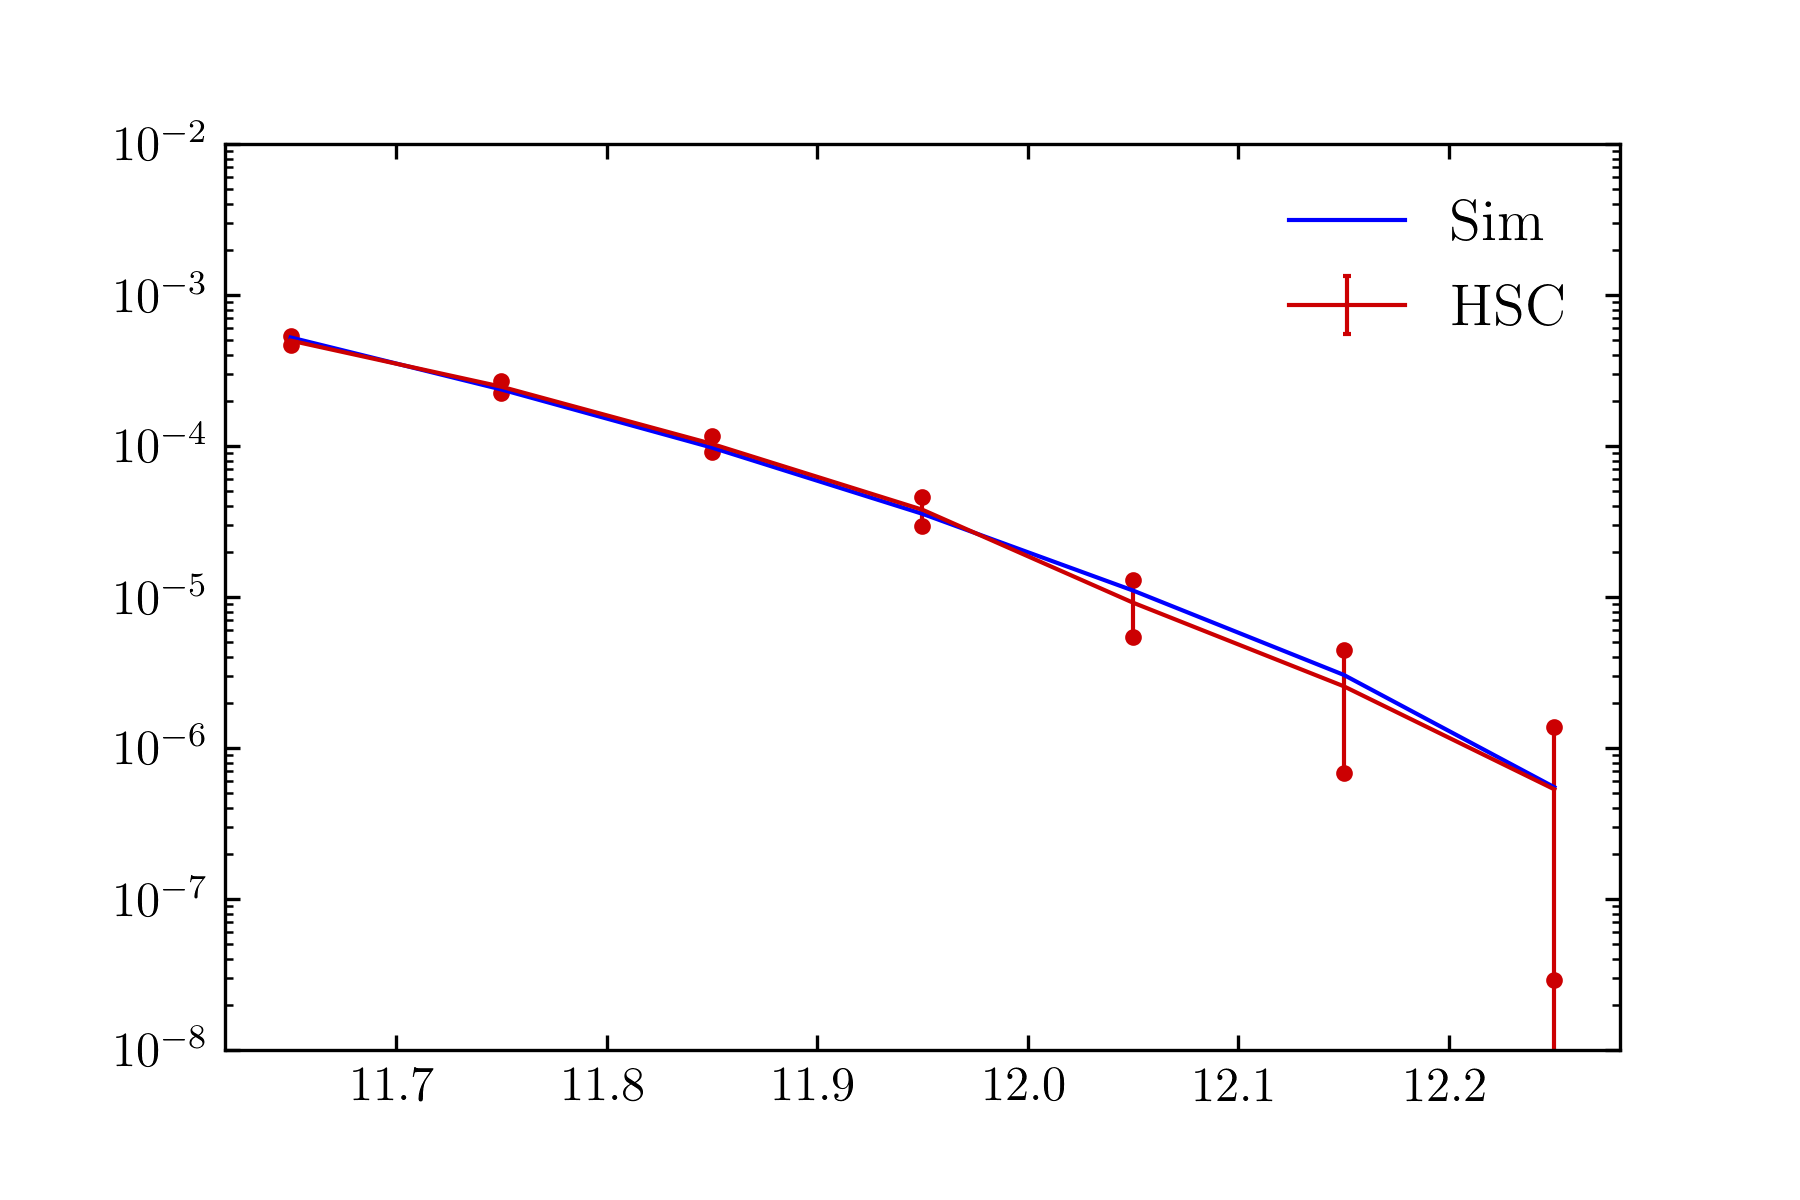
\includegraphics[width=\textwidth]{images/fit_smf.png}
        \end{figure}
    \end{block}


    \column{0.5\textwidth}
    \begin{block}{\MhaloPeak{}}
        \begin{figure}
        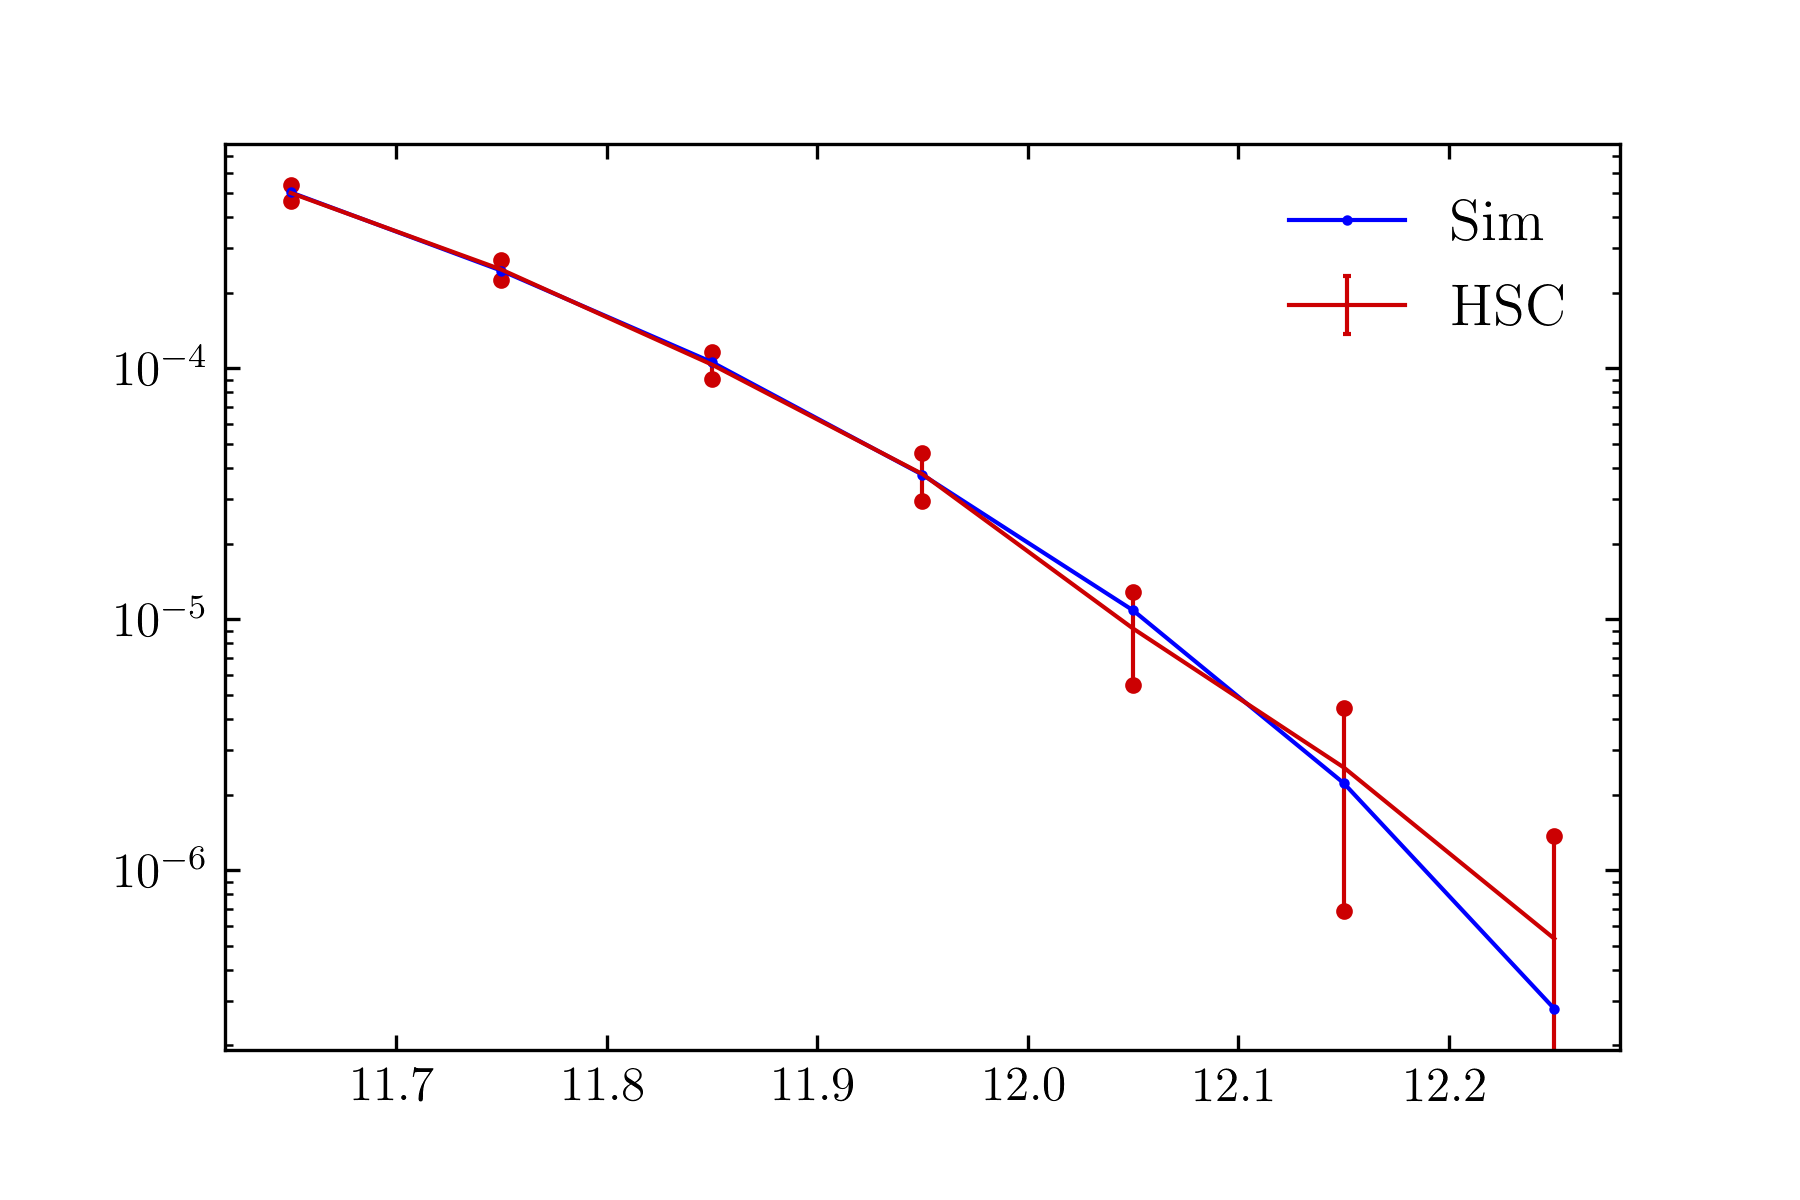
\includegraphics[width=\textwidth]{images/fit_smf_mpeak.png}
        \end{figure}
    \end{block}
    \end{columns}

\end{frame}



\begin{frame}
    \frametitle{Bestfit Models 2: Clustering}

    \begin{columns}
    \column{0.5\textwidth}

    \begin{block}{\vmp{}}
        \begin{figure}
        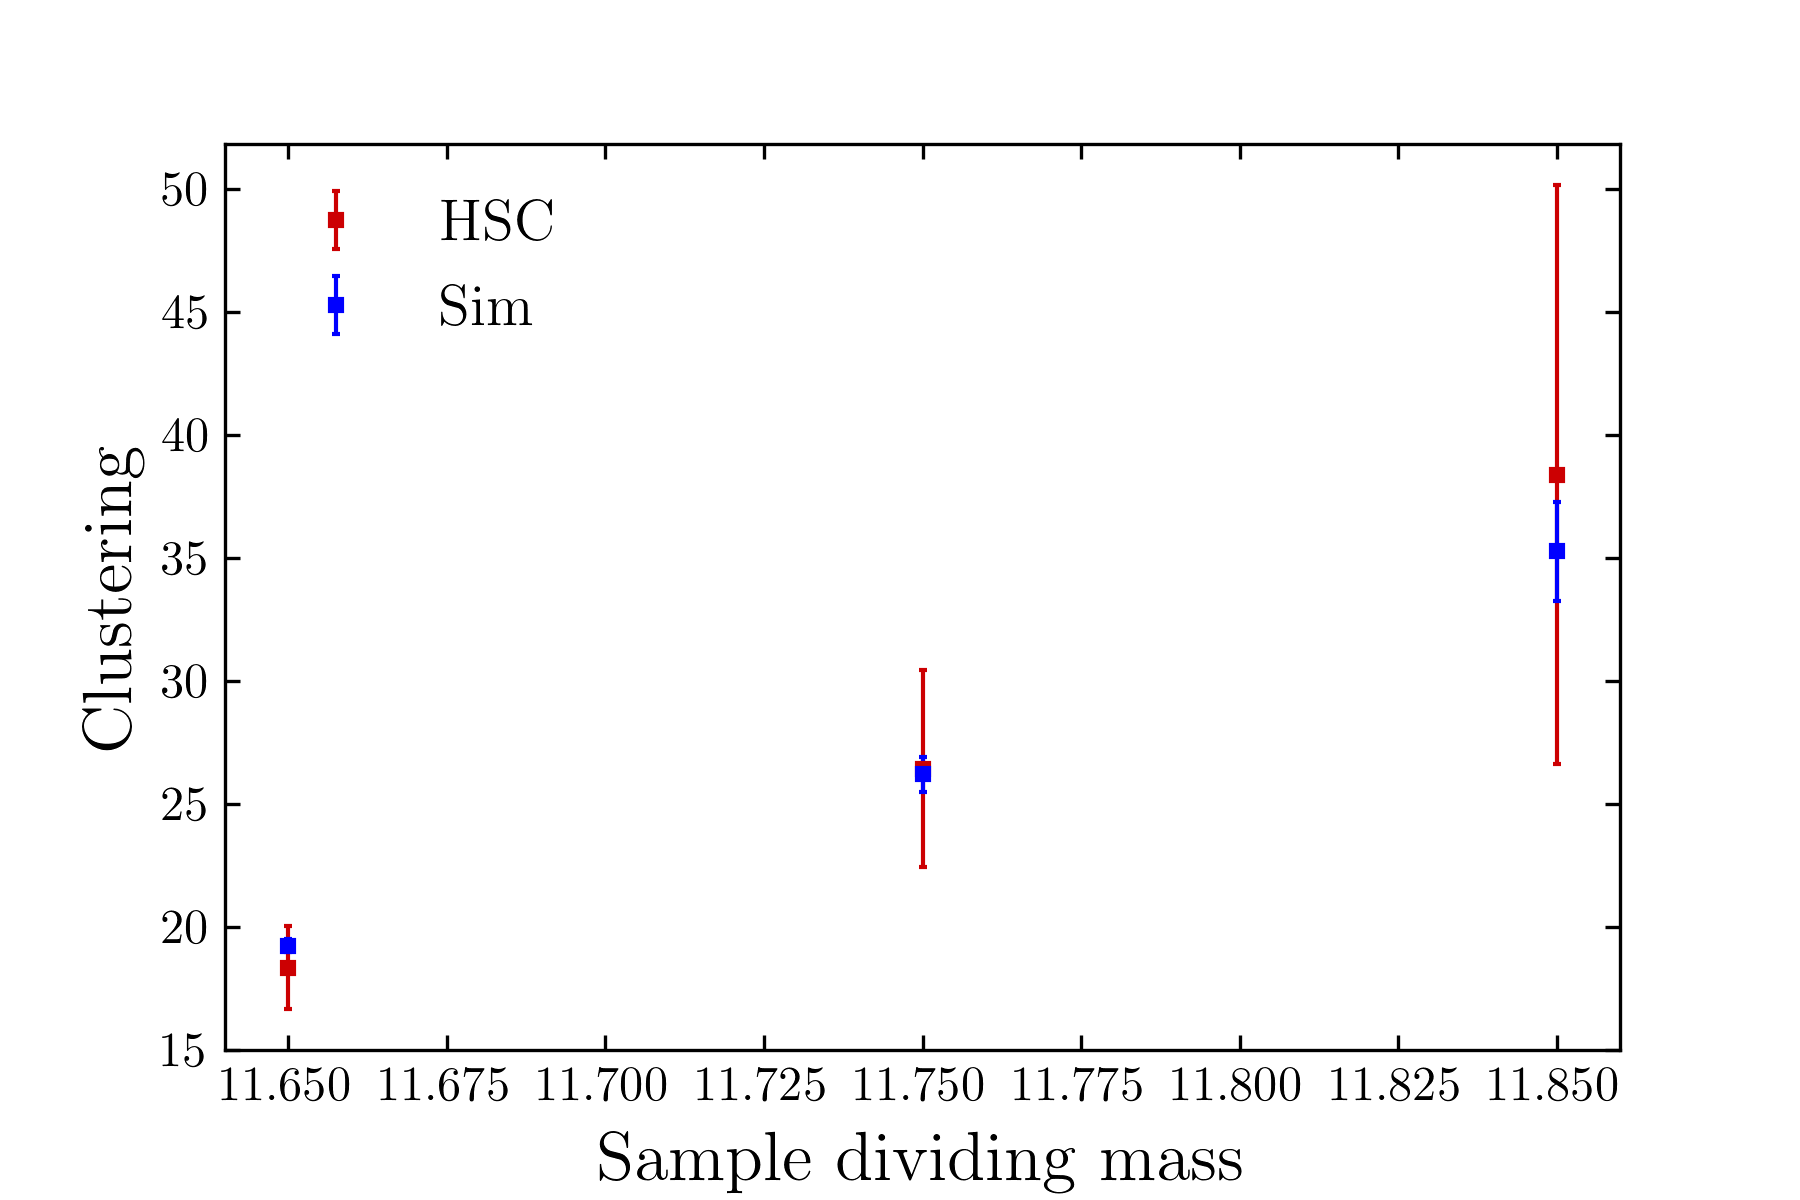
\includegraphics[width=\textwidth]{images/fit_clust.png}
        \end{figure}
    \end{block}


    \column{0.5\textwidth}
    \begin{block}{\MhaloPeak{}}
        \begin{figure}
        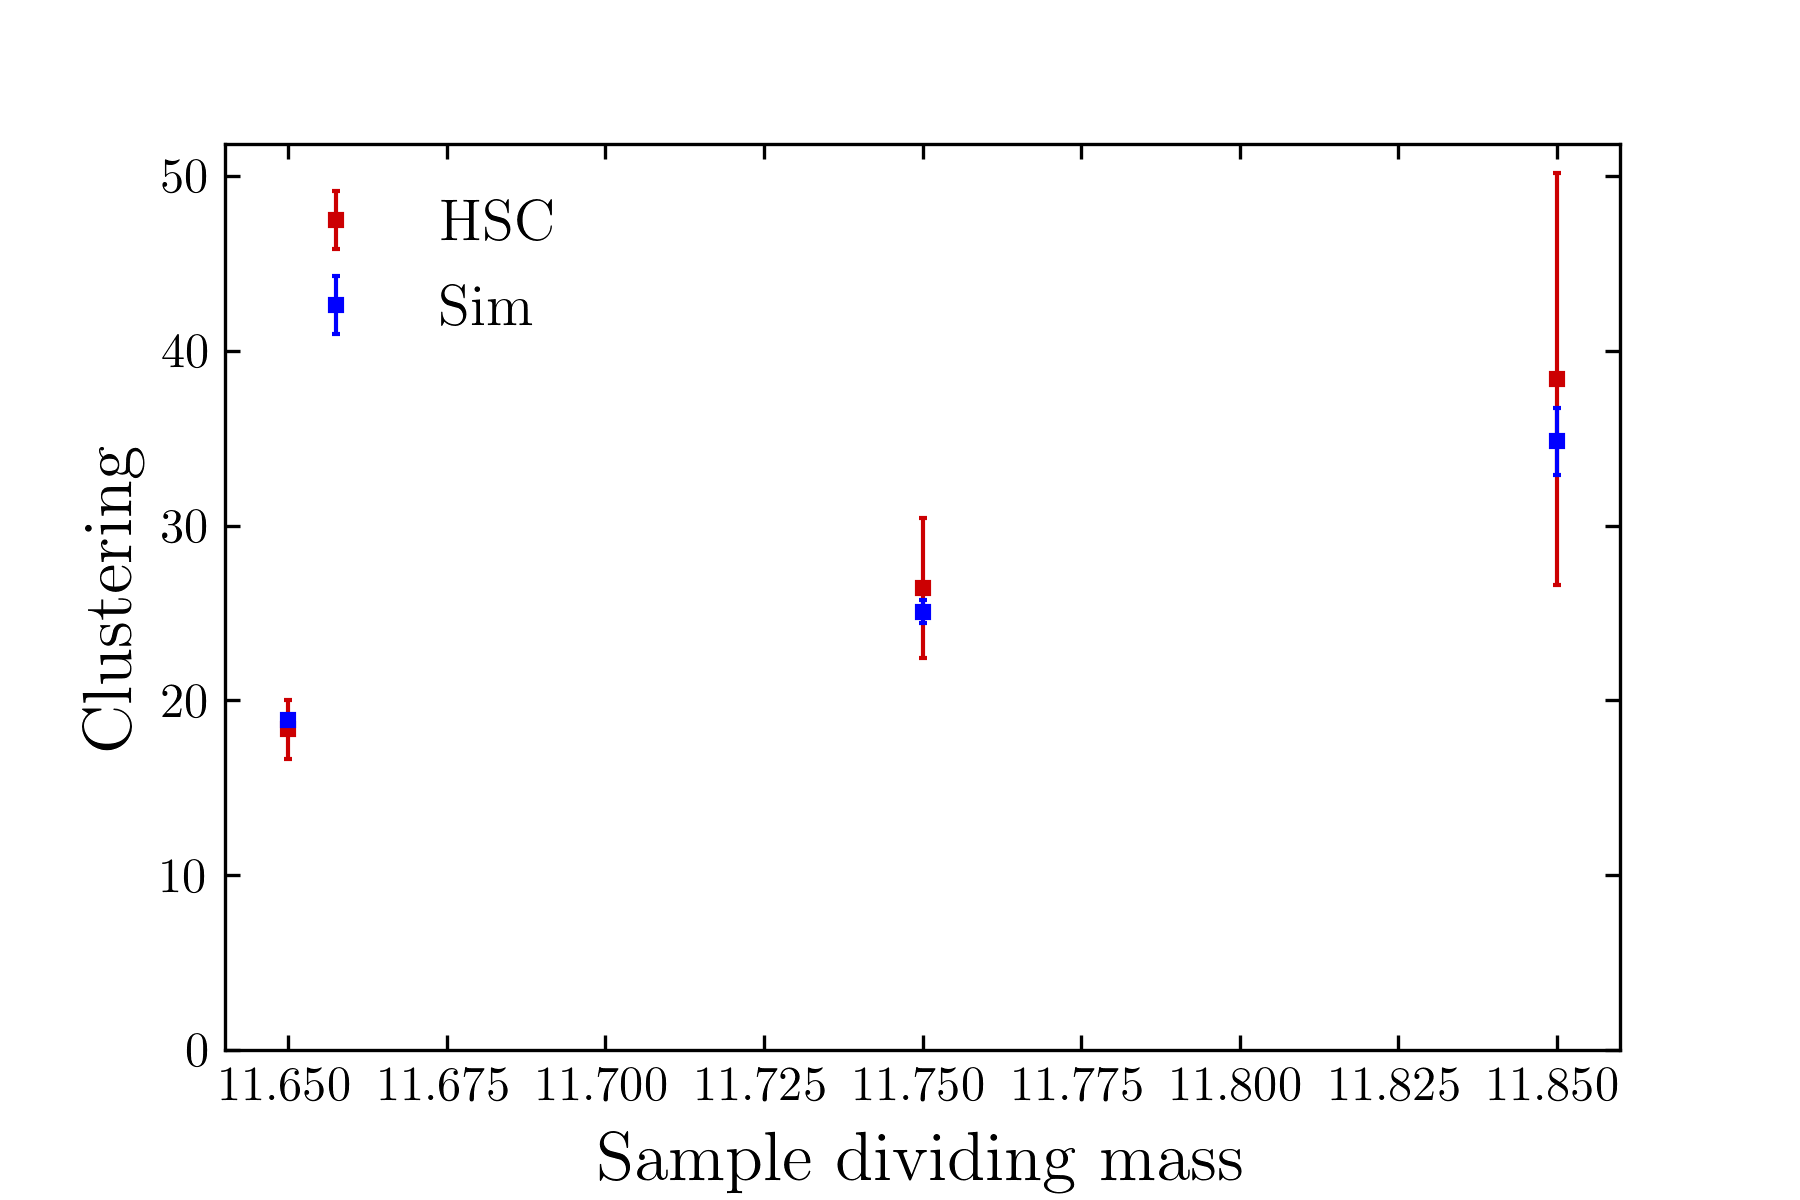
\includegraphics[width=\textwidth]{images/fit_clust_mpeak.png}
        \end{figure}
    \end{block}
    \end{columns}
\end{frame}

\begin{frame}
    \frametitle{Results 1: \fsat{}}

    \begin{figure}
    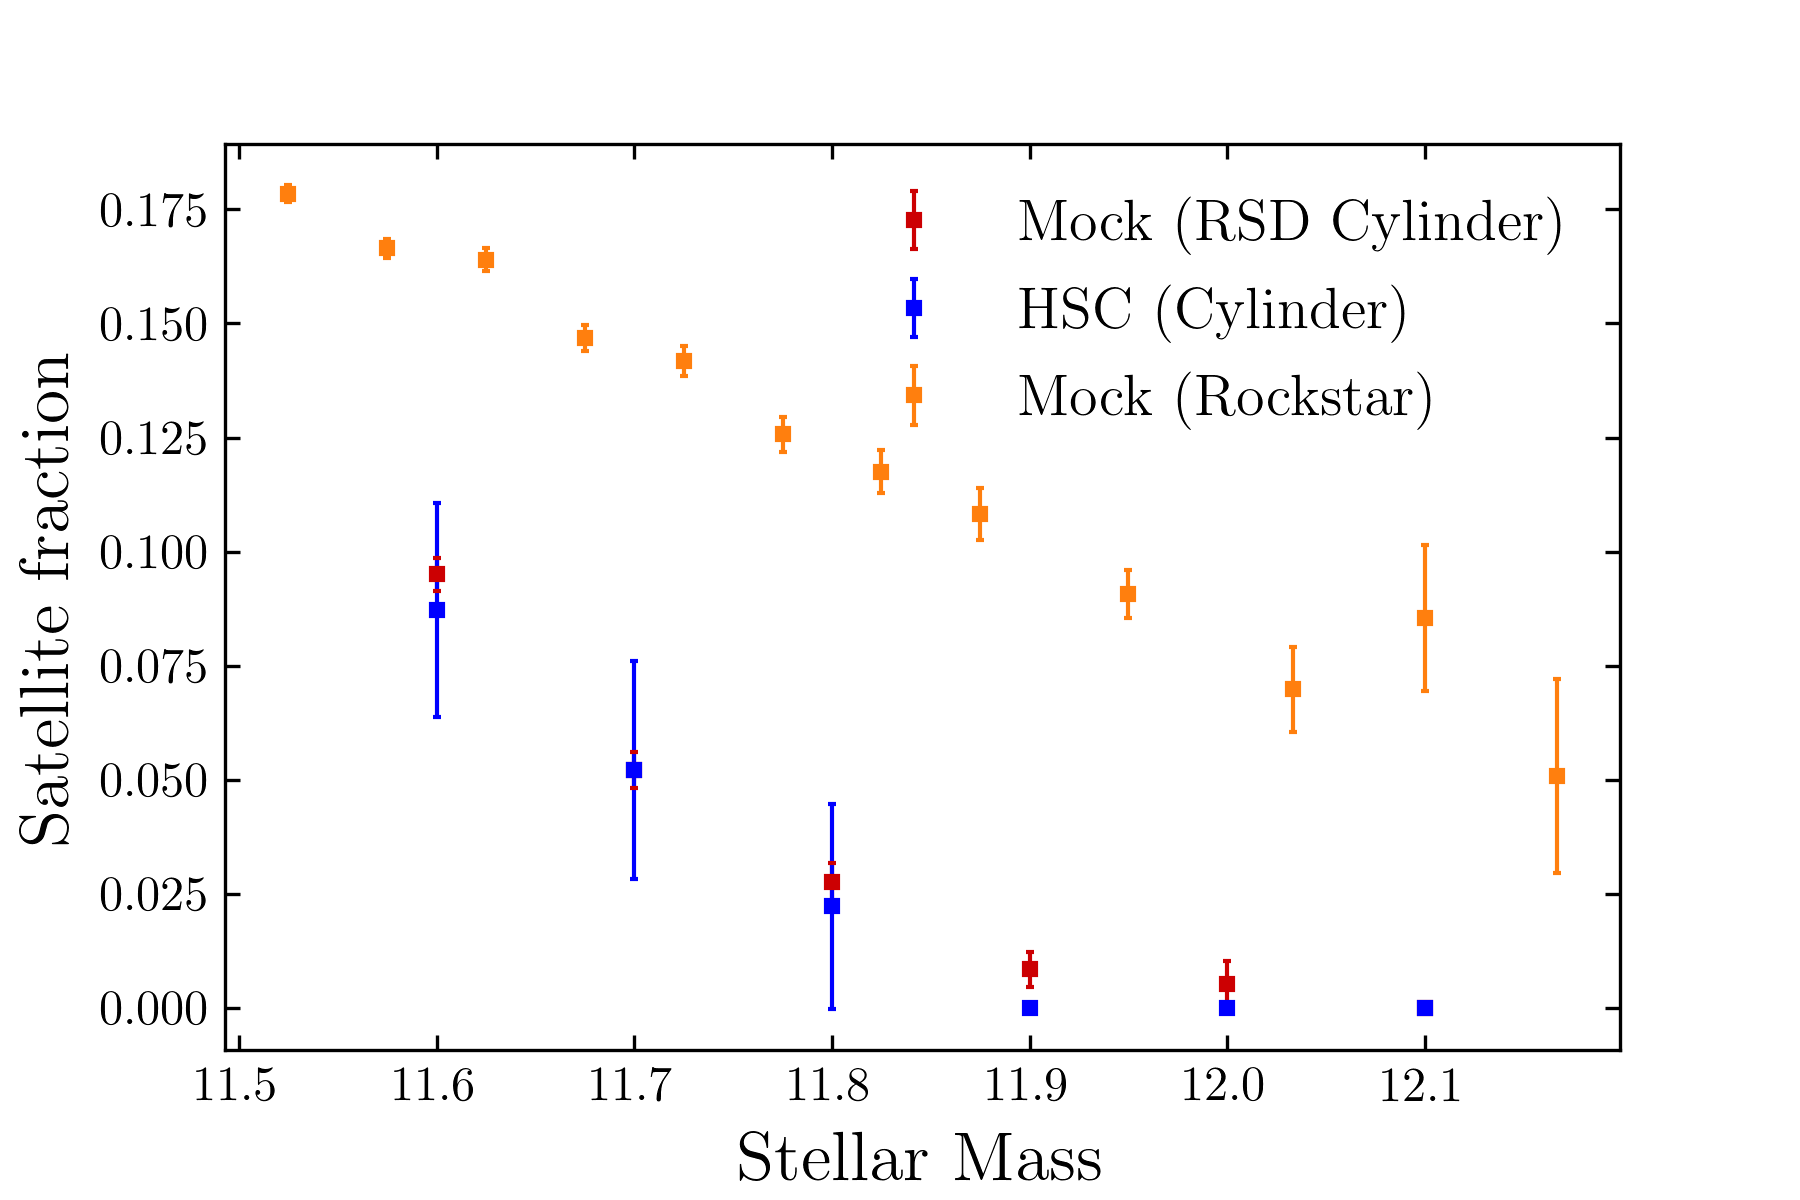
\includegraphics[width=0.9\textwidth]{images/sat_frac.png}
    \caption{Error bars show only the statistical error in all cases except Reddick+ 2013.}
    \end{figure}
\end{frame}

\begin{frame}
    \frametitle{Questions}
    \begin{itemize}
        \item I don't use any covariances in my best fit. This is certainly wrong though unclear how important?
        \item Auto vs cross correlation in the counts in cells stage?
    \end{itemize}
\end{frame}


\end{document}
